\chapter{Itération~0}
\label{sec:sprint0}

%\section*{Introduction}
%\addcontentsline{toc}{section}{Introduction}

L'itération 0 était dédiée à la présentation du projet aux membres de l'équipe,
à la recherche des choix technologiques, à la mise en place et au test de
l'environnement de développement. L'itération 0 a inclue des multiple des
réunions avec le directeur du produit (Product Owner) et des multiples
intervenants impliqués dans le produit pour la pré-planification du projet et
la préparation du carnet du produit nommé Backlog Général.

%Avant de commencer la première itération du Scrum, une période de temps à été
%consacrée pour préparer ce qui est nécessaire pour le lancement du projet dans
%des bonnes conditions. Cette période est souvent nommée l'itération 0 du
%projet. Elle est dédiée généralement à la recherche bibliographique, aux choix
%technologiques et à la mise en place de l'environnement de développement. Dans
%cette itération nous définissons le Backlog général de notre projet, ainsi que
%l'environnement du travail que nous avons besoin.

\section{Planification de l'itération}
La planification de l’itération représente une étape importante dans la vie de
l’itération parce que au cours du planification, on divise l’itération a plusieurs
tâches pour mieux atteindre le résultats attendu à la fin de l’itération.
\subsection{Répartition des rôles }
Chaque projet utilisant la méthode Scrum est monté autour d'une équipe
auto-organisée et multifonctionnelle: auto-organisée car il n'y a pas de chef
d'équipe qui décide les rôles de chacun, ou de la manière dont un problème est
résolu, puisque ces problématiques sont traitées par l'équipe dans son
ensemble; et multifonctionnelle car chaque membre de l'équipe forme une partie
prenante dans le développement de chaque fonctionnalité depuis l'idée jusqu'à
l'implémentation finale.

Dans Scrum existe trois principaux rôles:

\begin{itemize}
    \item Le responsable produit (Product owner).
    \item Le Scrum Master.
    \item Les membres de l'équipe.
\end{itemize}
\begin{figure}[!h]
    \centering
    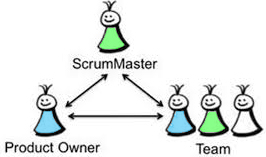
\includegraphics[width=.6\textwidth]{sprint0-scrum}
    \caption{}
    \label{fig:sprint0-scrum}
\end{figure}
\subsubsection{Le responsable produit \textquote{Product Owner}}

Il prend en charge de communiquer la vision globale du produit à l'équipe. Il
se voit représenter le client final, se met à sa place et priorise ses besoins.
Celui qui tient ce rôle est celui qui a le plus de visibilité, de
responsabilité et d'autorité. En effet, la méthode Scrum favorise
l'auto-organisation de l'équipe.

\subsubsection{Le Scrum Master}

Il joue le rôle du communiquant entre le responsable produit et l'équipe. Il ne
gère pas l'équipe, mais veille à éliminer tous les obstacles qui peuvent
empêcher l'équipe d'atteindre les objectifs fixés au cours d'un Sprint. En
résumé, ce rôle permet à l'équipe de rester créative et productive, tout en
veillant à ce que les réalisations soient visibles pour le responsable produit.

\subsubsection{Les membres de l'équipe  }

Dans la méthode Scrum, l'équipe est responsable de la réalisation
opérationnelle des itérations. L'équipe est généralement composée de personnes
multitâches. C'est toute l'équipe qui est responsable du résultat final de
chaque itération. La manière dont sont exécutées les tâches est très libre mais
cette liberté doit être néanmoins cadrée par l'obligation de répondre aux
objectifs du l'itération.

\subsection{Scrum Board}

Au cours de l'itération, on a utilisé Excel et un tableau physique pour suivre
l'évolution des tâches de chaque membre.

Dans les figures~\ref{fig:sprint1-fig1},~\ref{fig:sprint1-fig2}
et~\ref{fig:sprint1-fig2}, on représente l'état du tableau des tâches en jour
de distribution les tâches, au milieu et à la fin de l'itération
respectivement. Les lignes colorés représentent nos tâches du binôme. Les
colonnes du tableau sont:

\begin{description}
    \item [Who] L'allias du nom de chaque membres de l'équipe.

        \emph{Exemple:} \textbf{RM} signifie \textbf{R}ihab \textbf{M}ajdoub.
    \item [À faire (Todo)] Les tâches assignés au membres pour cette itération.
        L'échange des tâches entre les membres est possible sur le supervision
        du Scrum Master.
    \item [Implémentation] La pourcentage de l'implémentation du tâche de 0\%
        jusqu'à 100\%. Si le développeur a commencé l'implémentation d'une
        tâche, il la déplace dans cette colonne et faire le mise à jour du
        pourcentage de l'implémentation à chaque jour pendant un court réunion
        nommée \textquote{Daily Scrum} pendant le, on discute l'évolution du
        travail et le plan du jour prochain.
    \item [Test/Intégration/Review] L'implémentation du tâche est complete,
        elle est donc en phase d'évaluation et vérification de son
        fonctionnement si intégré dans le reste du système. Depuis la deuxième
        itération, au moins un autre membre doit revue le code pour à fin
        d'assurer la qualité du code, détecter et corriger les défauts le plus
        tôt possible.
    \item [Complete (Done)] La tâche était implémentée et validée.
\end{description}

On a utilisé des différents couleurs pour différents types des tâches:

\begin{description}
    \item [Rose] Les tâches du développement d'interface web (Dashboard).
    \item [Verte] Les tâches du développement mobile (l'application Android).
    \item [Jaune] Les tâches du développement des services web et d'administration.
\end{description}

La liste des prochaines réunions est écrite dans le tableau aussi:

\begin{itemize}
    \item Présentations des recherches si la tâche inclue une partie du
        recherche et présentation.
    \item Rendez-vous avec des autres personnes concernés par le projet.
    \item Si un développeur est besoin d'aide ou de discuter un problème
        rencontré.
    \item Code Revue à la fin d'itération fait par tous les membres pour
        évaluer la qualité du code et détecter les défauts du conception et
        d'implémentation.
\end{itemize}

\begin{figure}[H]
    \centering
    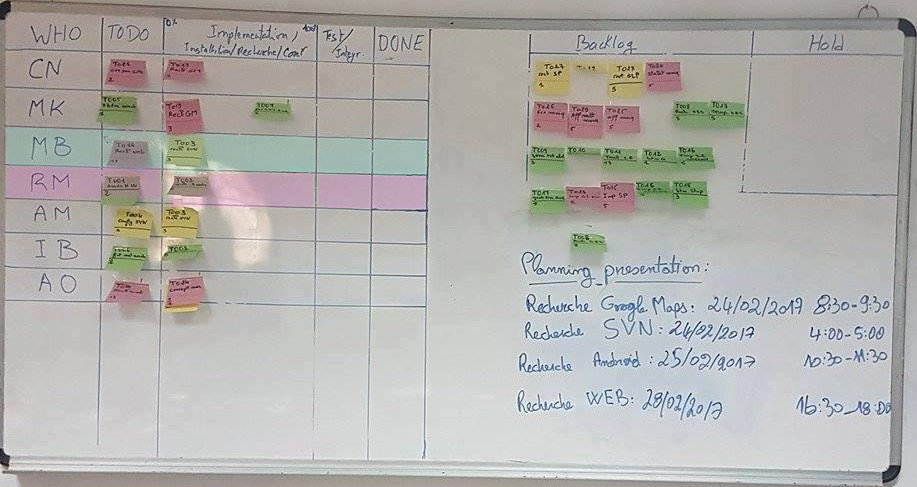
\includegraphics[width=0.9\textwidth]{sprint1-fig1}
    \caption{Logo du \textquote{Évolution du travail}}
    \label{fig:sprint1-fig1}
\end{figure}
%\begin{figure}[H]
%    \centering
 %   \caption[Évolution du travail --- Itération 0]{Évolution du travail}
    %\begin{subfigure}{0.5\linewidth}
        %\centering
        %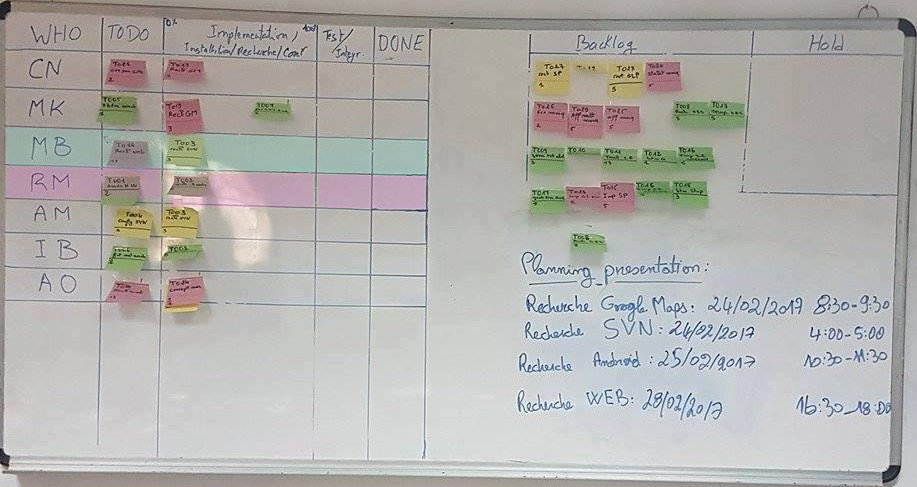
\includegraphics[width=0.9\linewidth]{sprint1-fig1}
        %\caption{Distribution des tâches de l'itération}
%\label{fig:sprint1-fig1}
    %\end{subfigure}

    %\begin{subfigure}{0.5\linewidth}
        %\centering
        %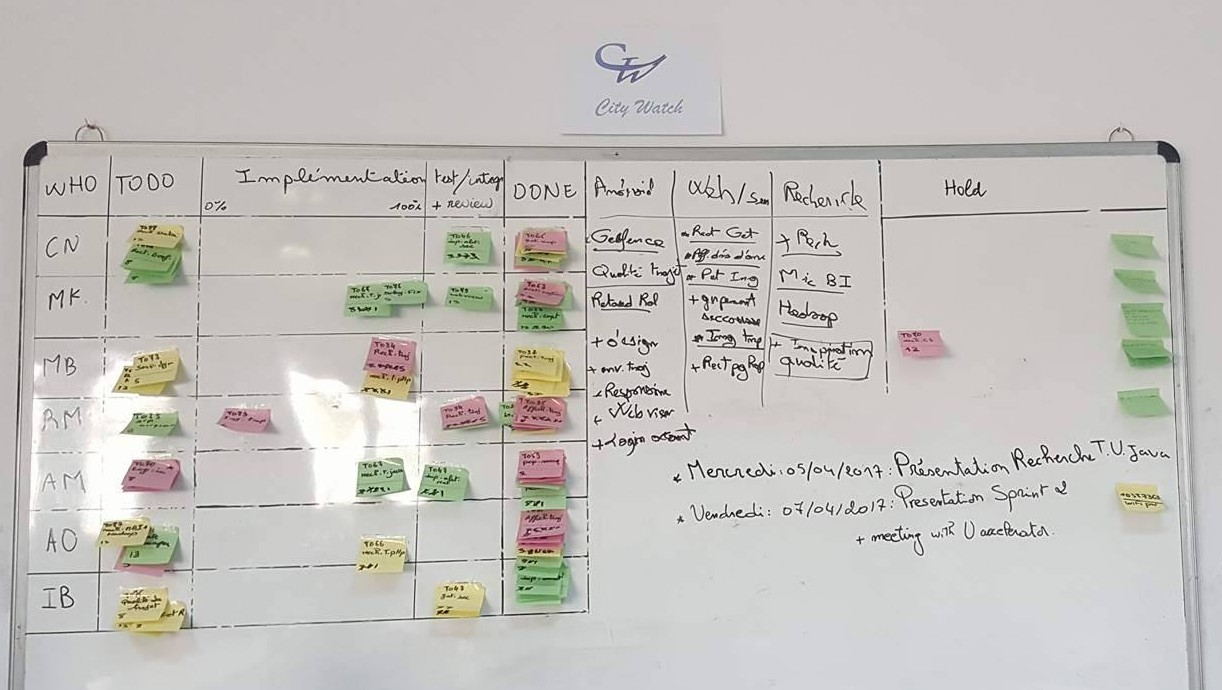
\includegraphics[width=0.9\linewidth]{sprint1-fig2}
        %\caption{Au milieu d'itération}
%\label{fig:sprint1-fig2}
    %\end{subfigure}

%    \begin{subfigure}{0.5\textwidth}
%        \centering
%        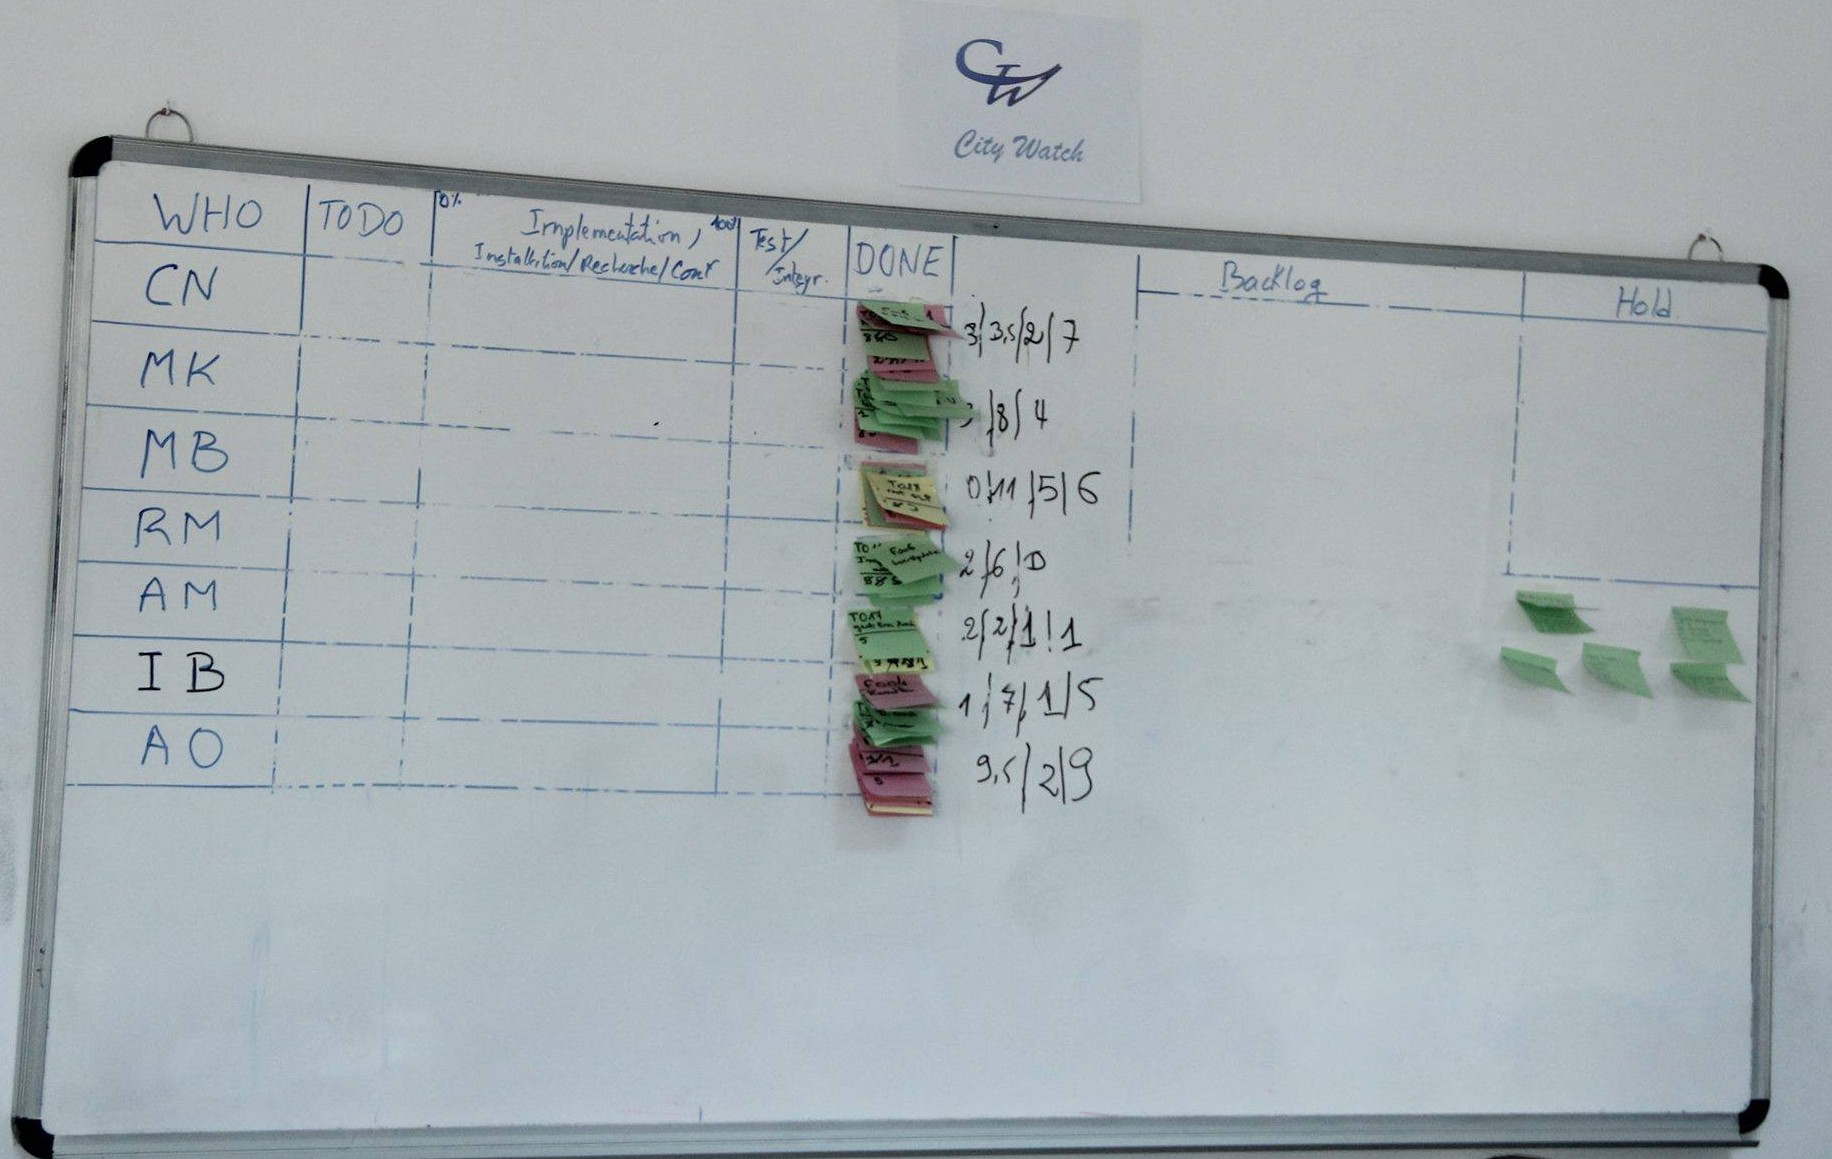
\includegraphics[width=0.9\linewidth]{sprint1-fig3}
%        \caption{Au fin d'itération}
%\label{fig:sprint1-fig3}
%    \end{subfigure}
%\end{figure}
\subsection{Burndown Chart}
Pour montrer l'avancement durant une itération donnée, on a besoin de tracer le
Burndown Chart. Il s'agit d'un graphique simple qui montre le nombre d'heures
restant à effectuer pour finaliser le produit.

\section{Backlog général}

La première étape de la méthode Scrum consiste à préparer un carnet du produit
(Product Backlog) qui présente la liste des tâches à effectuer durant le
développement du projet qui sera répartie en des itérations. Le Product Owner
prend en charge de communiquer la vision globale du produit à l'équipe. Il se
voit représenter le client final, se met à sa place et priorise ses besoins
selon des critères respectant la mission et les objectifs de son produit. En
précisant la valeur de priorité, il estime l'impact et le retour sur
investissement qu'aura chacun des items dans le carnet du produit. Il y a donc
effectivement eu un gros travail d'échanges et discussions avec le client pour
comprendre tout le cahier des charge initial, C'est comme ça que le Backlog a
été défini.

Les fonctionnalités qu'on a décidé d'implanter dans le projet \textquote{City Watch} inclut
un système itinéraire qui détecte la position et le trajet d'utilisateur,
un système d'information routière qui collecte les donnes sur l'infrastructure et
l'état de la route, un système de gestion des rapport qui permet de déclaré différents
type des rapport, un système de capture des information réseaux cellulaires,
un système
d'analyse est de valorisation qui projeté ces données instantanément
en des cartographie et des diagramme dynamique et configurable et un système d'assistance
qui guide et notifie l'utilisateur.


La figure~\ref{fig:product-backlog} présente une version simplifiée du Product
Backlog complète des 3 premières itérations. Nous représentons notre
participation de binôme par les cercles du texte souligné.

\usetikzlibrary{mindmap,shadows}
\newcommand*{\info}[4][16.3]{%
  \node [ annotation, #3, scale=0.65, text width = #1em,
          inner sep = 2mm ] at (#2) {%
  \list{$\bullet$}{\topsep=0pt\itemsep=0pt\parsep=0pt
    \parskip=0pt\labelwidth=8pt\leftmargin=8pt
    \itemindent=0pt\labelsep=2pt}%
    #4
  \endlist
  };
}
\begin{figure}[htbp]
%\usepackage{dtklogos}
\hspace{-9ex}
\begin{tikzpicture}[every annotation/.style={draw, fill=white, font=\Large}]
    \renewcommand{\href}[2]{#2}

    \path[mindmap,
          concept color=black!40,
          text=white,
          every node/.style={
              concept,
              circular drop shadow,
              execute at begin node=\hskip0pt,
          },
          %grow cyclic,
          root/.style={
              concept color=black!40,
              fill=white, line width=1ex, text=black,
              font=\footnotesize\bfseries,
              text width=7em},
          level 1 concept/.append style={
              font=\normalsize\bfseries,
              sibling angle=50,
              text width=7.7em,
              level distance=12.5em,
              inner sep=0pt},
          level 2 concept/.append style={
              font=\footnotesize\bfseries,
              level distance=8em},
          ours/.append style = {
              line width=0.5ex,
              concept color = black,
          }
    ]

    node[root] {Platforme CityWatch} [clockwise from=0]

    child[concept color=blue!70] {
        node {\ul{Gestions des Rapports}} [clockwise from=50]
        child { node { \ul{Consultation} } }
        child { node { \ul{D\'eclaration} } }
    }
    child[concept color=green!40!black] {
        node[concept] {\ul{Information Routi\`ere}} [clockwise from=30]
        child { node[concept] {\ul{Secousses}} }
        child { node[concept] {\ul{Ralentisseurs}}}
        child { node[concept] {Embouteillage}}
    }
    child[concept color=blue] {
        node[concept] {\ul{Itin\'eraire}} [clockwise from=305]
        child { node[concept] {\ul{Localisation instantan\'e}} }
        child { node[concept] {\ul{Projection du Trajectoire}} }
        child { node[concept] {\ul{Historie des Trajectoires}} }
    }
    child[concept color=red!60!black] {
        node[concept] {Assistance} [clockwise from=235]
        child { node[concept] {Alerte des secousses} }
        child { node[concept] {Alerte des ralentisseurs} }
    }
    child[concept color=orange] {
        node[concept] {\ul{Tableau de Bord}} [counterclockwise from=100]
        child { node[concept] {\ul{Carte en Temps R\'eel}}}
        child { node[concept] {\ul{Authentification}} }
        child { node[concept] {\ul{Filtrages}} }
    }
    child[concept color=yellow!60!black] {
        node[concept] (Blogs) {\ul{Analyse et Visualisation}} [clockwise from=135]
        child { node[concept] {Visualisation des données}}
        child { node[concept] {\ul{Tableau du bord interactive}}}
    }
    child[concept color=red] {
        node[concept] {Information Réseau} [clockwise from=110]
        child { node[concept] {Signal Réseau} }
        child { node[concept] {Génération Réseau} }
        child { node[concept] {Opérateur Réseau} }
    };
\end{tikzpicture}
\caption{Objective du produit}
\label{fig:product-backlog}
\end{figure}


Le tableau~\ref{tab:product-backlog} représente une liste plus détaillé des cas
d'utilisations que nous allons implémentés pendant les 3 premières itérations.
La définition des ces cas d'utilisation suivre la forme:

\begin{displayquote}
    En tant que \textbf{X}, je peux \textbf{Y} Afin d'\textbf{Z}.
\end{displayquote}

Ou aussi la forme:

\begin{displayquote}
    En tant que \textbf{X}, je veux qu'il soit possible de \textbf{Y} pour
    \textbf{Z}.
\end{displayquote}

Ou \textbf{X} est l'acteur initiateur, \textbf{Y} est le service rendu par le
système et \textbf{Z} est le but du cas. Prenant comme example le cas
d'utilisation suivant: En tant qu'utilisateur, je veux qu'il soit possible de
localiser ma position continuellement pour l'afficher instantanément sur une
cartographie.

Dans notre liste des cas
d'utilisation, l'acteur initiateur (\textbf{X}) est toujours l'utilisateur.

Les valeurs des priorités de cas d'utilisation sont définies comme le suivants:

\begin{description}[align=right,labelwidth=1cm]
    \item [1:] Définie une haute priorité, affectée pour les spécifications
        importantes, exigées pour le produit.
    \item [2:] Définie une priorité importante mais pas exigée.
    \item [3:] Définie une priorité moyenne ou parfois faible.
\end{description}

\Needspace{5\baselineskip}
\begin{center}
    \footnotesize
    \setlength\LTleft{-20pt}
    \begin{longtable}{| l | p{3.5cm} | p{5.5cm} | p{5cm} | l |}
        \caption{Backlog du Produit}
        \label{tab:product-backlog} \\

        \hline
        \textbf{ID} & \textbf{Cas d'utilisation} & \textbf{Je veux qu'il soit possible de} & \textbf{Pour} & \textbf{Priorité} \\ \hline
        \endhead

        \hline \multicolumn{5}{|r|}{{Continué en page suivante$\dotsc$}} \\ \hline
        \endfoot

        \hline \hline
        \endlastfoot

        \hline
1 & Gestion du Trajectoire & Activer le localisation & Enregistrer le trajectoire & 1 \\ \cline{3-5}
&                          & Consulter le dashboard  & Afficher le trajectoire instantané & 1 \\ \cline{3-5}
&                          & Filtrer le trajectoire  & Consulter l'histoire des trajectoires & 2 \\ \hline
2 & Gestion des Rapports   & Déclarer un rapport depuis le site & Avoir un rapport dans la carte & 1 \\ \cline{3-5}
&                          & Choisir un emplacement & Afficher et filtrer par catégorie & 1 \\ \cline{3-5}
&                          & Ajouter une image et commentaire & Enrichir le rapport & 1 \\ \cline{3-5}
&                          & Accéder à formulaire depuis l'application mobile & rapporter instantané et facilement & 2 \\ \cline{3-5}
&                          & Activer/Désactiver le groupement des marqueurs & Avoir une vision sur le nombre des rapports plus claire & 3 \\ \hline
3 & Tableau de bord (Dashboard) & Consulter le dashboard & Visualiser diffèrent type de données comme marqueurs et zones & 1 \\ \cline{3-5}
&                               & Manipuler la légende   & Filtrer les données affichés & 1 \\ \hline
4 & Comptes                & Créer un compte & Pouvoir enregistrer des données personnels (trajectoire) & 3 \\ \cline{3-5}
&                          & Se connecter & Accéder au données routières privées (trajectoire) & 3 \\ \cline{3-5}
&                          & Visiter le dashboard sans compte & Consulter une version minimale des fonctionnalités & 3 \\
        \hline
    \end{longtable}
\end{center}

\section{Préparation de l'environnement du travail}

Pendant l'itération 0, on a fait un recherche sur les choix techniques à fin de
mettre en place l'environnement de développement. Ces choix concernent
l'environnement logiciel à utiliser tel que les langues de programmations, les
frameworks et les outils de développement.
% , ainsi, la listes des besoins matériels.

% \subsection{Environnement logiciel}

La réalisation de ce projet nécessite l'ensemble de ces plateformes et
frameworks que nous allons cités:

\subsection{Développement Application Mobile avec Android}

Android est un système d'exploitation basé sur le noyau Linux ciblant
principalement les smartphones, les tablettes avec support pour les
technologies mettables, les télévisions et les voitures. Il est le système
mobile le plus utilisé dans le monde avec 88\% de part de marché des
smartphones en Novembre 2016~\cite{android-market-share}.

Le système économique d'Android est très fort avec plus de 2,950,000
d'applications~\cite{android-apps} en Google Play Store en
Mai 2017. Jusqu'à Mai 2017, la dernière version majeure du système Android est
Nougat (7.X) disponible depuis le mois d'aout 2016~\cite{android-7-release}
avec le dernier mise à jour est 7.1.2 disponible le 5 janvier 2017.

On a choisi du supporter le système Android comme notre première plateforme. Ce
choix était basé sur différents aspects:

\begin{itemize}
    \item La part de marché des smartphones et tablettes Android.
    \item L'ouverture de la plateforme, et l'accessibilité aux différentes
        fonctionnalités et aux outils de développements.
    \item Android Auto, Android Wear, Android Things\ldots
\end{itemize}

Android Studio (v2.3) était le choix naturel pour le développement
d'application grâce au support officiel du Google et les fonctionnalités
héritées de l'ide IntelliJ IDEA de JetBrains comme un concepteur d'interface
utilisateur pour des résolutions variées simultanément, débogueur, \ldots.

Dans la première itération, cette partie va être encore élaborée pour faire le
choix adéquat de la version de SDK à utiliser puisque les versions du système
Android en marché supportent des variétés des SDKs qui peuvent être riches en
fonctionnalités et le choix de la version de SDK dépend de ces fonctionnalités
à utiliser.

\subsection{Développement Web}

En se basant sur les conseils du Product Owner et aux limites d'environnement
de développement dont le serveur supporte seulement PHP, on a choisi la langue
de programmation PHP (PHP 7.0).

Les points fort de la langue PHP:

\begin{itemize}
    \item Une langue très répondu dans le développement Web, Elle a une
        grande communauté des développeurs.
    \item Une grande liste des outils de développement incluant les
        gestionnaires des dépendances (Composer, Phar), outils des tests
        unitaires (PHPUnit), générateurs du documentation (PHPDoc, Sami),
        débogueurs (Xdebug), analyseurs du code et analyseurs statiques
        (php\_CodeSniffer, PHPLint), outils d'automatisation (Phing) and
        multiple IDEs.
    \item Multiple bibliotheques et frameworks pour différent type des projets.
\end{itemize}

Les points faibles de la langue PHP:

\begin{itemize}
    \item Gestion d'erreurs très souple par défaut même si les erreurs sont
        fatales.
    \item Manque d'un paradigme unique dans l'architecture de la langue (le
        choix du syntaxe et du noms des fonctions)
\end{itemize}

L'ide choisie pour le développement PHP est PHPStorm (2017.1),
un IDE multiplatforme de JetBrains. Il regroupe sous une interface conviviale
un éditeur de texte avancé et intelligent, un interpréteur et un
débogueur\ldots. Vim a été aussi utilisé avec un ensemble des extensions pour
enrichir ses fonctionnalités.

Au coté client, on dépend des technologies Web modernes qui nous permttre de
créer une application web interactive et dynamique rapidement et aisément sans
besoin d'un backend pour générer le contenu.

\begin{description}
    \item [HTML 5.1] On a utilisé les tags sémantique, les nouveaux types et
        attributes de validations des entrés du formulaire et les nouveautés
        des api Web comme l'api DOM et l'api de localisation.
    \item [CSS 3] Ou plus précisément les modules stabilisés du CSS niveau 3.
        \TODO{used indirectly throw Bootstrap 3/4 + materielize css}
    \item [JavaScript 7] Ou encore ECMAScript 2016\textregistered
        définit dans la spécification ECMA-262 \cite{ECMA262}. On a utilisé le
        programmation POO, la programmation asynchrone (Promise) et des autres
        nouveautés de syntaxe.
\end{description}

L'utilisation de ces dernières mise à jours des standards du web a causé que
notre application web est supporté par seulement les dernières versions des
navigateurs principales\footnote{Firefox v45+ (sans support d'input de type
date), Google Chrome v50+, Edge v14+, Sfari 10+ (sans support d'input de type
date), Opera 37}. Le support des autres anciennes versions et des autres
navigateurs était possible en demande à travers les transcompilateurs du
ECMAScript 2016+ à ECMAScript 5.1 comme Babel ou Traceur même si il n'était pas
une priorité pendant notre phase de développement. Quelques fonctionnalités de
ECMAScript 2016 n'étaient pas utilisées car elles ne sont pas encore
implémentées par aucun des navigateurs principales comme les Modules.

\subsection{Environnement matériel}

Pour le développement de ce projet, il était demandé d'avoir:

\begin{itemize}
    \item Serveur Local pour les tests
        \begin{itemize}
            \item Windows 10
            \item Wamp Server 3.0
            \item Apache 2.4
            \item PHP 7.0
            \item MySQL 5.7
        \end{itemize}
    \item Serveur de production:
        \begin{itemize}
            \item Linux
            \item Accès FTP
            \item Apache 2.4
            \item PHP 7.0
            \item MySQL 5.5
        \end{itemize}
\end{itemize}

\section*{Conclusion}
\addcontentsline{toc}{section}{Conclusion}

L'itération 0 nous a permis de bien comprendre le produit à développer et de
préparer le terrain pour une bonne entame de développement. Pendant cette
itération, nous avons élaboré le carnet de notre projet avec la collaboration
du Product Owner.
